%
% Capítulo 2
%
\chapter{Arquitetura e tecnologias} \label{cap:arquitetura}

O presente capítulo pretende expor uma visão geral da organização técnica do projeto, os diferentes módulos que o compõem e suas intedependências, bem como as linguagem de programação e \textit{frameworks} usadas no seu desenvolvimento.\\

\section{Visão geral do sistema} \label{arquitetura:visão}
O projeto encontra-se dividido em dois blocos principais, \textit{frontend} e \textit{backend}, interligados entre si. \\

\begin{figure}[h]
	\centering
	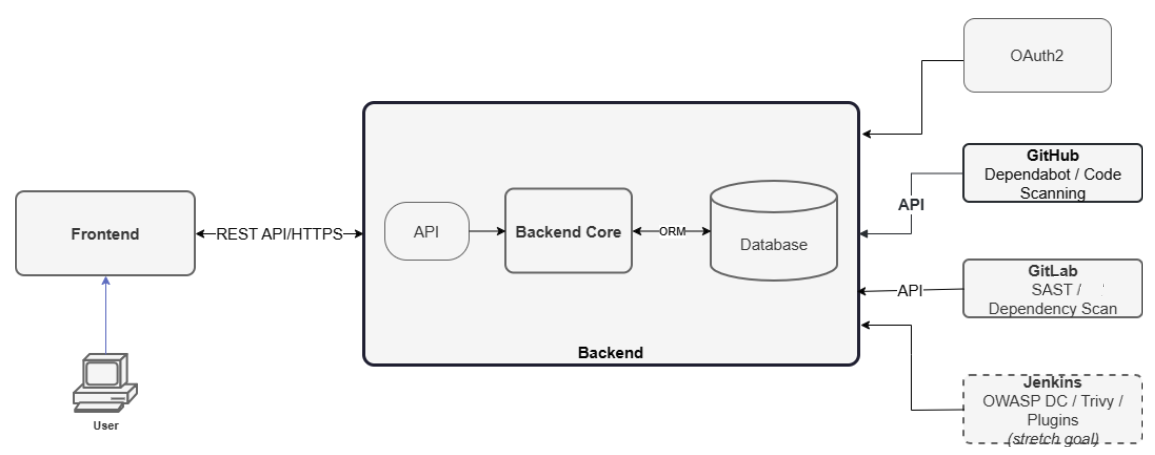
\includegraphics[width=0.75\linewidth]{./figures/diagrama.png}
	\caption{caption teste}
\end{figure}

O \textit{backend} é o principal responsável pela lógica de negócio da aplicação, recaindo nele as funções de comunicar com as APIs externas às quais a aplicação necessita de recorrer e de normalizar a informação recebida destas. É também sua responsabilidade toda a lógica de registo e autorização dos utilizadores e a persistências dos dados numa base de dados. O \textit{backend} atua também como uma \textbf{API REST}, expondo os dados necessários de forma estruturada via pedidos \textbf{HTTP}. \\

Enquanto isso, o \textit{frontend} constitui a interface visual com que o utilizador interage via web browser. O seu papel é consumir os dados enviados pelo \textit{backend} e exibí-los ao utilizador de forma interativa através de uma página web, tratando de toda a lógica de navegação e visualização. \\

Esta separação modular, tendo por base o princípio de \textit{separation of concerns}, para além de permitir escolhas técnicas mais especializadas para cada módulo, reduz a complexidade ao limitar a interação entre estes, permitindo que cada camada evolua de forma independente, facilitando a manutenção e atualização futura do sistema. \\

Para além disso, separar a lógica de apresentação da lógica de dados permite que uma única API, implementada no \textit{backend} venha a servir potenciais múltiplas plataformas (web, desktop, mobile, etc). \\


\section{APIs externas} \label{arquitetura:apis}
O funcionamento da aplicação está intrinsecamente ligado ao usp de APIs externas.  Os utilizadores podem-se autenticar através da utilização do protocolo \textit{OAuth 2.0} usando como \textit{identity providers} Google, GitHub ou GitLab. \\

Estes dois últimos provedores de identidade cumprem um papel duplo, pois para além da possibilidade de providenciarem \textit{autenticação} ao SecDash são também eles que providenciam \textit{autorização}, de forma a que a aplicação possa requisitar os repositórios dos utilizadores bem como consumir os endpoints de segurança que contêm os relatórios de vulnerabilidades sobre os quais a funcionalidade base do projeto assenta. \\

\section{Tecnologias e linguagens} \label{arquitetura:tecnologias}
\subsection{Backend} \label{arquitetura:tecnologias:backend}
\subsection{Frontend} \label{arquitetura:tecnologias:frontend}